% ============================================================================
%  BLOQUE VII — DIAPOSITIVAS 25–26: DEMOSTRACIÓN PRÁCTICA
% ============================================================================
\section{Demostración}

% ----------------------------------------------------------------------------
%  DIAPOSITIVA 25 — VÍDEO DE DEMOSTRACIÓN (layout 2 columnas)
% ----------------------------------------------------------------------------
\begin{frame}{Demostración: Test de Integración Completa}
  \begin{columns}[T]
    \column{0.55\textwidth}
    \centering
    \begin{exampleblock}{Panel multimedia}
      \centering
      \IfFileExists{captura_demo.png}{%
        \movie[width=0.95\textwidth, height=6.4cm, poster, showcontrols]{%
          \begin{tikzpicture}
            \node[inner sep=0] (img) {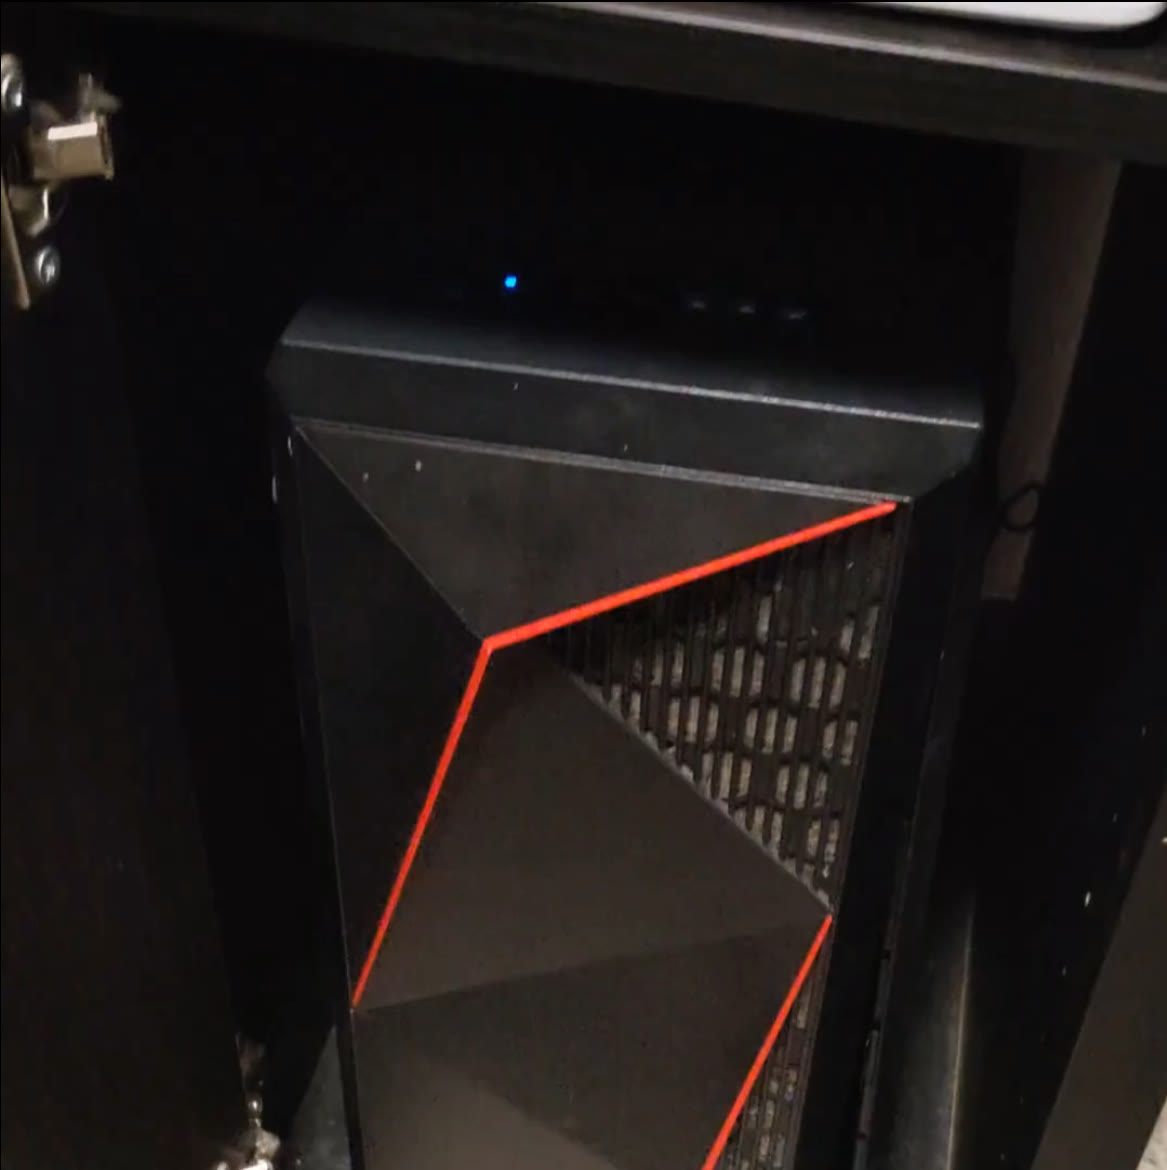
\includegraphics[width=0.95\textwidth, height=6.4cm,
              keepaspectratio]{captura_demo.png}};
            \fill[primary, opacity=0.7] (img.center) circle (0.7cm);
            \node[white, font=\Huge\bfseries] at (img.center) {$\blacktriangleright$};
          \end{tikzpicture}%
        }{video_demo.mp4}
      }{%
        \fbox{\parbox{0.85\textwidth}{\centering
          \vspace{2cm}
          \textcolor{primary}{\Huge $\blacktriangleright$}\\[0.2cm]
          {\large\bfseries\color{primary}VÍDEO DE DEMOSTRACIÓN}\\[0.1cm]
          {\footnotesize\color{darkgray}\texttt{captura\_demo.png} + \texttt{video\_demo.mp4}}
          \vspace{2cm}
        }}
      }
    \end{exampleblock}

    \column{0.45\textwidth}
    \begin{alertblock}{Protocolo de Contingencia}
      \scriptsize
      \textbf{Respaldo 1 — Local}\\[0.1cm]
      \centering
      \href{run:video_demo.mp4}{\beamergotobutton{Abrir archivo local}}\\[0.15cm]
      {\scriptsize\texttt{video\_demo.mp4}}

      \vspace{0.3cm}
      \textbf{Respaldo 2 — YouTube}\\[0.1cm]
      \centering
      \href{https://youtu.be/\_\_rJUlpLXP4}{\beamergotobutton{Ver en YouTube}}\\[0.15cm]
      {\scriptsize\texttt{youtu.be/\_\_rJUlpLXP4}}\\[0.2cm]
      \qrcode[height=0.8cm]{https://youtu.be/\_\_rJUlpLXP4}
    \end{alertblock}
  \end{columns}
\end{frame}

% ----------------------------------------------------------------------------
%  DIAPOSITIVA 26 — TELEGRAM + DASHBOARD
% ----------------------------------------------------------------------------
\begin{frame}{Demostración Práctica: Telegram + Dashboard}
  \sloppy
  \begin{columns}[T]
    \column{0.42\textwidth}
    \IfFileExists{\memoriaimg/hw_telegram_chat.jpg}{%
      
\includegraphics[height=4.3cm, keepaspectratio]{\memoriaimg/hw_telegram_chat.jpg}%
    }{%
      \fbox{\parbox{0.9\textwidth}{\centering\footnotesize [Chat Telegram]}}%
    }\\[0.1cm]
    {\footnotesize Conversación real con Luxe Core AI vía Telegram}

    \column{0.58\textwidth}
    \IfFileExists{\memoriaimg/hw_dashboard.png}{%
      
\includegraphics[height=4.3cm, keepaspectratio]{\memoriaimg/hw_dashboard.png}%
    }{%
      \fbox{\parbox{0.9\textwidth}{\centering\footnotesize [Dashboard OpenClaw]}}%
    }\\[0.1cm]
    {\footnotesize Dashboard web de OpenClaw (\texttt{http://192.168.1.50:18789})}
  \end{columns}

  \centering
  \footnotesize
  \textbf{Comandos en lenguaje natural}\\
  $\rightarrow$ interpretados en local\\
  $\rightarrow$ ejecución en hardware real.\\
  Ningún mensaje abandona la subred.
\end{frame}
